\documentclass{BHCexam}
\biaoti{~$2012 - 2013$~学年度期末考试}
\fubiaoti{高二数学试卷}
\usepackage{palatino}
\usepackage{siunitx}%输入度数符号需要的单位宏包
\usepackage{tikz}
\usetikzlibrary{shapes.geometric, arrows}
\tikzstyle{startstop} = [rectangle, rounded corners, minimum width = 1cm, minimum height=0.5cm,text centered, draw = black]
\tikzstyle{io} = [trapezium, trapezium left angle=70, trapezium right angle=110, minimum width=0.5cm, minimum height=0.5cm, text centered, draw=black]
\tikzstyle{process} = [rectangle, minimum width=2cm, minimum height=0.5cm, text centered, draw=black]
\tikzstyle{decision} = [diamond, aspect = 2, text centered, draw=black]
% 箭头形式
\tikzstyle{arrow} = [->,>=latex]
\zihao{-4}

\begin{document}
\maketitle
\mininotice

\begin{questions}

%选择题
\xuanze
\qs 已知命题~$p:\exists x\in \mathbf{R}$~,使~$\sin x=\dfrac{5}{2}$~;命题~$q:\forall x\in \mathbf{R}$~,都有~$x^2+x+1>0$~下列结论中正确的是\xx.\\
\twoch{命题是“$p\wedge q$”真命题}{命题是“$p\wedge \neg q$”真命题}{命题是“$\neg p\wedge q$”真命题}{命题是“$\neg p\vee \neg q$”假命题}

\qs 在~$\triangle ABC$~中,“$A>B$”是“$\sin A> \sin B$”的\xx.\\
\twoch{充要条件}{必要不充分条件}{充分不必要条件}{既不充分也不必要条件}
\qs 在同一坐标系中,方程~$a^2x^2+b^2y^2=1$~与~$ax+by^2=0(a>b>0)$~的曲线大致是\xx.\\
\begin{center}
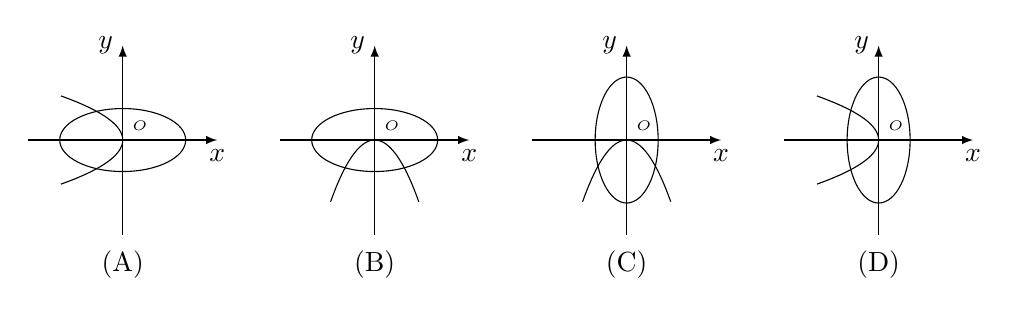
\begin{tikzpicture}[scale=0.8]
\coordinate[label=above right:\tiny $O$] (O) at(0,0);
\draw[->,>=latex](-1.5,0)--(1.5,0)node[below](x){$x$};
\draw[->,>=latex](0,-1.5)--(0,1.5)node[left](y){$y$};
\draw (0,0) ellipse (1cm and 0.5cm);
\draw[domain=-0.7:0.7,samples=1000,rotate=90] plot (\x,{2*(\x)^2});
\coordinate[label=below:$(\mathrm{A})$](A)at (0,-1.6);
\begin{scope}[xshift=4cm]
\coordinate[label=above right:\tiny $O$] (O) at(0,0);
\draw[->,>=latex](-1.5,0)--(1.5,0)node[below](x){$x$};
\draw[->,>=latex](0,-1.5)--(0,1.5)node[left](y){$y$};
\draw (0,0) ellipse (1cm and 0.5cm);
\draw[domain=-0.7:0.7,samples=1000,rotate=180] plot (\x,{2*(\x)^2});
\coordinate[label=below:$(\mathrm{B})$](B)at (0,-1.6);
\end{scope}
\begin{scope}[xshift=8cm]
\coordinate[label=above right:\tiny $O$] (O) at(0,0);
\draw[->,>=latex](-1.5,0)--(1.5,0)node[below](x){$x$};
\draw[->,>=latex](0,-1.5)--(0,1.5)node[left](y){$y$};
\draw (0,0) ellipse (0.5cm and 1cm);
\draw[domain=-0.7:0.7,samples=1000] plot (\x,{-2*(\x)^2});
\coordinate[label=below:$(\mathrm{C})$](C)at (0,-1.6);
\end{scope}
\begin{scope}[xshift=12cm]
\coordinate[label=above right:\tiny $O$] (O) at(0,0);
\draw[->,>=latex](-1.5,0)--(1.5,0)node[below](x){$x$};
\draw[->,>=latex](0,-1.5)--(0,1.5)node[left](y){$y$};
\draw (0,0) ellipse (0.5cm and 1cm);
\draw[domain=-0.7:0.7,samples=1000,rotate=-90] plot (\x,{-2*(\x)^2});
\coordinate[label=below:$(\mathrm{D})$](D)at (0,-1.6);
\end{scope}
\end{tikzpicture}
\end{center}
\qs 已知变量~$x,y$~满足条件 $\begin{cases}
x\geq 1 \\
y\leq 2  \\
x-y\leq 0  \\
\end{cases}$,则目标函数$z=2x+y$的最小值是\xx.\\
\onech{$2$}{$3$}{$4$}{$6$}
\qs 如果$\log_3{m}+\log_3{n}=4$,则$ m+n $的值依次为\xx.\\
\onech{$ 4\sqrt{3} $}{$ 4 $}{$ 9 $}{$ 18 $}
\qs 在等差数列~$\left\{ a_n \right\}$~中,$ a_1=-25,S_3=S_8$~,则前~$n$~项和~$S_n$~的最小值为\xx.\\
\onech{$ -74 $}{$ -75 $}{$ -76 $}{$ -80 $}
\qs 函数$ f(x) $的定义域为~$(a,b)$,导函数$ f'(x) $在$ (a,b) $内的图象如图所示,则函数$ f(x) $在~$(a,b)$~内的极大值点有\xx.\\
\fourch{$ 1\text{个} $}{$ 2\text{个} $}{$ 3\text{个} $}{$ 4\text{个}$}
\vspace{-4cm}
\begin{flushright}
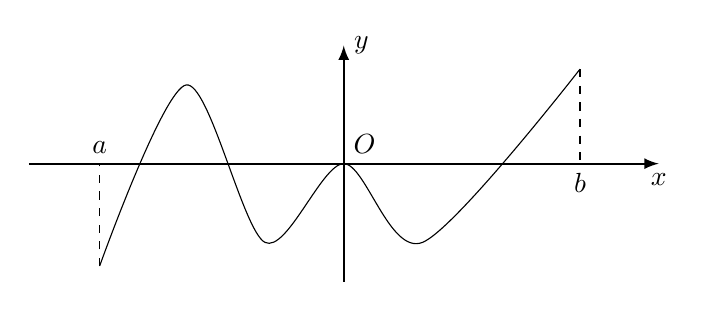
\begin{tikzpicture}
\draw[->,>=latex, thick] (-4,0)--(4,0) node[below] at (4,0) {$x$};
\draw[->,>=latex, thick] (0,-1.5)--(0,1.5) node[right] at (0,1.5) {$y$};
\draw plot[smooth] coordinates {(-3.1,-1.3)    (-2,1)    (-1,-1)  (0,0)  (1,-1)  (3,1.2)};
\draw[dashed] (3,1.2)--(3,0) node[below] at (3,0) {$b$};
\draw[dashed] (-3.1,-1.3)--(-3.1,0) node[above] at (-3.1,0) {$a$};
\node[above right] at (0,0) {$O$};
\end{tikzpicture}
\end{flushright}
\qs 直线$ y=kx+2 $与抛物线~$y^2=8x$~有且只有一个公共点,则~$k$~的值为\xx.\\
\onech{$ 1$}{$ 1\text{或} 3$}{$ 0$}{$ 1~\text{辆} 0$}
\qs 定义:数列~$\{a_n \}$~前~$n$~项的积~$T_n=a_1\cdot a_2\cdot\, \cdots\, \cdot a_n$~,数列~$a_n=2^{9-n}$~,则下面等式中正确的是\xx.\\
\onech{$T_1=T_{19}$}{$T_3=T_{17}$}{$T_5=T_{12}$}{$T_8=T_{11}$}
\qs (非城区学生做)已知双曲线的顶点与焦点分别是椭圆$\dfrac{x^2}{a^2}+\dfrac{y^2}{b^2}=1(a>b>0)$~的焦点与顶点,若双曲线的离心率为$2$~,则椭圆离心率为\xx.\\
\onech{$\dfrac{1}{3}$}{$\dfrac{\sqrt{3}}{3}$}{$\dfrac{1}{2}$}{$\dfrac{\sqrt{2}}{2}$}
(城区学生做)已知点~$P$~在曲线~$C_1:\dfrac{x^2}{16}-\dfrac{y^2}{9}=1$~上,点~$Q$~在曲线~$C_2:(x-5)^2+y^2=1$~上,点~$R$~在曲线~$C_3:(X+5)^2+y^2=1$~上,则~$\abs{PQ}-\abs{PR}$~的最大值是\xx.\\
\onech{$6$}{$8$}{$10$}{$12$}

请把选择题答案写在下表里:\\%
\begin{tabular}{|c|c|c|c|c|c|c|c|c|c|c|}
\hline
题号&~~~~1~~~~&~~~~2~~~~&~~~~3~~~~&~~~~4~~~~&~~~~5~~~~&~~~~6~~~~&~~~~7~~~~&~~~~8~~~~&~~~~9~~~~&~~~~10~~~~  \\
\hline
答案&&&&&&&&&&  \\
\hline

\end{tabular}
%填空题
\tiankong
\qs 命题“存在一个无理数,它的平方是有理数”的否定是\ltk.
\qs 不等式$\dfrac{x-1}{x}\geq 2$~的解集为\ltk.
\qs 已知等差数列~$\{a_n \}$~的前~$n$~项和为~$S_n=(a+1)n^2+a$~,某三角形之比为~$a_2:a_3:a_4$~,则该三角形最大内角为\ltk.
\qs 在等比数列~$\{a_n \}$~中,若~$a_3=\dfrac{3}{2},S_3=\dfrac{9}{2}$~,则公比~$q$~的值等于\ltk.
\qs (非城区学生做)下列结论正确的是\ltk.写出所有正确结论的序号)\\
\ding{192}常数列既是等差数列,又是等比数列;\\
\ding{193}若数列~$\{a_n \}$~的前~$n$~项和为~$S_n=n^2+n+1$~,则~$\{a_n \}$~的通项公式~$a_n=2n+1$~;\\
\ding{194}若数列~$\{a_n \}$~的前~$n$~项和为~$S_n=3^n-1$~,则~$\{a_n \}$~,则~$\{a_n \}$~为等比数列;\\
\ding{195}设~$x_1,x_2$~是关于~$x$~的方程~$\left| \log_a x \right|=k(a>0,a\neq 1)$~的两根,则~$x_1x_2=1$~。\\
(城区学生做)数列~$\{a_n \}$~中,如果对任意~$n\in \mathrm{N^*}$~都有~$\dfrac{a_{n+2}-a_{n+1}}{a_{n+1}-a_n}=k(k\text{为常数})$~,则称~$\{a_n \}$~为等差比数列,~$k$~称为公差比。现给出下列命题:\\
\ding{192}等差比数列的公差比一定不为~$0$~;\\
\ding{193}等差数列一定是等差比数列;\\
\ding{194}若~$a_n=-3^n+2$~,则数列~${a_n}$~是等差比数列;\\
\ding{195}若等比数列是等差比数列,则其公比等于公差比。\\
其中正确的命题的序号为\ltk.

%解答题
\jianda
\qs (12分)已知~$a,b,c$~分别是~$\triangle ABC$~的三个内角所对的边,若~$\triangle ABC$~面积~$S_{\triangle ABC}=\dfrac{\sqrt{3}}{2},c=2,A=60^{\circ}$~,求~$a,b$~的值。
\vspace{7cm}
\qs (12分)给定两个命题,$P:$对任意实数~$x$~都有~$ax^2+ax+1>0$~恒成立;$Q:$关于~$x$~的方程~$x^2-x+a=0$~有实数根;如果~$P$~与~$Q$~中有且仅有一个为真命题,求实数~$a$~的取值范围。

\vspace{7cm}
\qs (12分)已知过抛物线~$y^2=2px(p>0)$~的焦点~$F$~的直线交抛物线于$A(x_1,y_1),B(x_2,y_2)$两点。\\
求证:~$x_1\cdot x_2$~为定值。
\vspace{7cm}
\qs (非城区学生做13分)已知等差数列~$\{a_n \}$~满足:~$a_3=7,a_5+a_7=26,\{a_n \}$~的前~$n$~项和为~$S_n$~。
\begin{parts}
\part 求~$a_n$~及~$S_n$~;
\part 令~$b_n=\dfrac{1}{a_n ^2-1}(n\in N^*)$~,求数列~$\{b_n \}$~的前项和~$T_n$~。
\end{parts}
(城区学生做13分)已知数列~$\{a_n \}$~满足条件:~$a_1=t,a_{n+1}=2a_n+1$~。
\begin{parts}
\part 判断数列~$\{a_n+1 \}$~是否为等比数列;
\part 若~$t=1$~,令~$b_n=\dfrac{2^n}{a_n\cdot a_{n+1}}$~,求数列~${b_n}$~的前~$n$~项和~$T_n$~。
\end{parts}
\vspace{8cm}
\qs (13分)已知函数~$f(x)=\dfrac{1}{3} x^3+\dfrac{1}{2} (b-1)x^2+cx$~($b,c$为常数)。
\begin{parts}
\part 若~$f(x)$~在~$x=1$~和~$x=3$~处取得极值,试求~$b,c$~的值;
\part 若~$f(x)$~在~$(-\infty,x_1),(x_2,+\infty)$~上单调递增,且在~$(x_1,x_2)$~上单调递减,又满足~$x_2-x_1>1$~。\\
求证:~$b^2>2(b+2c)$~;
\end{parts}
\newpage
\qs (非城区学生做13分)$P$为椭圆~$\dfrac{x^2}{25}+\dfrac{y^2}{9}=1$~上一点,$F_1,F_2$为左右焦点,若~$\angle F_1PF_2=60^{\circ}$~。
\begin{parts}
\part 求~$\triangle F_1PF_2$~的面积;
\part 求点~$P$~的坐标。
\end{parts}
(城区学生做13分)如图,椭圆~$G$~的中心在坐标原点,其中一个焦点为圆~$F:x^2+y^2-2x=0$~的圆心,右顶点是圆~$F$~与~$x$~轴的一个交点。已知椭圆~$G$~与直线~$l:x-my-1=0$~相交于~$A,B$~两点。
\begin{parts}
\part 求椭圆的方程;
\part 求~$\triangle OAB$~面积的最大值。
\end{parts}
\begin{flushright}
\begin{tikzpicture}
\tikzmath{
\a=-0.5*sqrt(7);
\b=0.4*sqrt(7);
\c=0.25*sqrt(7);
\d=-0.375*sqrt(7);
}
\draw[->,>=latex] (-2.5,0)--(2.5,0) node[below] at(2.5,0) {$x$};
\draw[->,>=latex] (0,-2)--(0,2) node[right] at(0,2) {$y$};
\draw (0,0) ellipse (2cm and 1cm);
\draw (1,0) circle (1cm);
\draw (0,\a)--(1.8,\b);
\node[below left] at(0,0) {$O$};
\node[below] at(1,0) {$F$};
\coordinate [label=right:$A$](A) at (1.5,\c);
\coordinate [label=right:$B$](B) at (0.25,\d);
\draw (0,0)--(A) (0,0)--(B);
\end{tikzpicture}
\end{flushright}

\end{questions}
\end{document}
